%!TeX program = xelatex
% VizDOM paper draft (IEEE conference format: ICST / AST / ICSE SEIP use IEEEtran;
% for ISSTA switch to acmart). Build: powershell -ExecutionPolicy Bypass -File build.ps1
%
% Section -> source mapping (where each part was drawn from):
%   I   Introduction          report/vizdom_report_en.tex sec. 1, docs/present slide 12c
%   II  Background            report sec. 2 (landscape, capability matrix)
%   III Lifecycle benchmark   benchmarks/README.md sec. 1-5, report sec:lifecycle
%   IV  VizDOM                report sec. 3-4 (arch, pipeline), sec:desc, ADR-022/024/027
%   V   Setup                 benchmarks/report_gpu_20261026_run3.html sec. 2 (PV config)
%   VI  Results               benchmarks/README.md sec. 6, run-3 report sec. 3-9
%   VII Threats               run-3 report sec. 10, report "Discussion and Limitations"
% Every number is traceable to a result JSON under benchmarks/results/ (gitignored;
% tarballs kept) by run id and commit, as listed in Table II.
\documentclass[conference]{IEEEtran}
\IEEEoverridecommandlockouts

\usepackage{cite}
\usepackage{amsmath,amssymb}
\usepackage{fontspec}            % XeLaTeX: IEEE's Times (system font on Windows/macOS;
\setmainfont{Times New Roman}    % on Linux/Overleaf use "TeX Gyre Termes" or \usepackage{newtxtext})
\usepackage{graphicx}
\usepackage{booktabs}
\usepackage{multirow}
\usepackage[table]{xcolor}
\usepackage{url}
\usepackage[hidelinks]{hyperref}

\graphicspath{{../report/figures/}}
\newcommand{\code}[1]{\texttt{#1}}
\newcommand{\todo}[1]{\textcolor{red}{[TODO: #1]}}
\def\BibTeX{{\rm B\kern-.05em{\sc i\kern-.025em b}\kern-.08em T\kern-.1667em\lower.7ex\hbox{E}\kern-.125emX}}

\begin{document}

\title{A Resolved DOM Can Say No:\\Screenshot-Derived Visual DOMs versus Vision--Language Grounders as GUI Test Oracles}

\author{
\IEEEauthorblockN{Nguyen Huynh Tri Cuong}
\IEEEauthorblockA{Faculty of Information Technology\\University of Science, VNU-HCM\\Ho Chi Minh City, Vietnam\\nhtcuong@gmail.com}
\and
\IEEEauthorblockN{Nguyen Van Vu}
\IEEEauthorblockA{Faculty of Information Technology\\University of Science, VNU-HCM\\Ho Chi Minh City, Vietnam\\\todo{email}}
}
% \todo{Confirm author order, affiliations (industrial affiliation?), and whether a
% publication clearance from the employer is required before submission.}

\maketitle

\begin{abstract}
GUI test automation needs two things from a perception layer: find the element a step refers to, and judge whether a step's expectation holds. Vision--language grounders, built for autonomous agents, are measured almost exclusively on the first. We ask whether they can serve the second. We present a lifecycle benchmark that runs every system under comparison on the same 514 locate--act--verify steps over 44 screen states, including 88 \emph{negative} verification steps whose target is deliberately absent, and scores a testing-specific \emph{false-pass} rate alongside action-hit and cost. On it we compare three end-to-end grounders (Aria-UI, ELAM-7B, UI-TARS-1.5-7B) with VizDOM, a system that parses a screenshot once into a UI-Automator-like Visual DOM and resolves every step against it under an exactly-one locator contract. The grounders click better (0.93--0.96 against 0.88) but pass 60 to 88 of the 88 absent targets; VizDOM passes none, by construction, at 15--39 times lower cost per step. With its own description-based language tier switched on, lexical scoring over the DOM with a 3B text model as tie-breaker, VizDOM exceeds ELAM's action-hit (0.934), reaches the best verification accuracy of the table (0.964) and still passes none of the 88 absent targets. The same experiment shows the failure is a property of the paradigm, not of model size: a 3B vision model placed behind the DOM's own candidate shortlist regains the hits and accepts 34 of 40, then 17 of 30, of the nonsense captions it is shown, and the 3B text model itself accepts 38 of 88 when asked over the whole DOM instead of a short list. The best clicker is the worst oracle, and the difference is structural: a per-step grounder is trained to always produce an answer, whereas a resolved DOM can say no.
\end{abstract}

\begin{IEEEkeywords}
GUI testing, test oracle, visual grounding, vision--language models, screenshot parsing, test automation
\end{IEEEkeywords}

% =====================================================================
\section{Introduction}
% =====================================================================
GUI test automation depends on one capability: finding an on-screen element and addressing it reliably across runs. Frameworks such as Appium and Selenium obtain this addressability from a platform accessibility tree \cite{uiautomator,appium}. A large class of applications exposes no such tree: custom-rendered desktop UIs (Qt/QML, OpenGL, game engines), embedded and industrial human--machine interfaces, and any screen observed through a camera or a capture card. For these, teams fall back to pixel coordinates or template images \cite{yeh2009sikuli}, which break on the first layout, theme or resolution change.

Two families of vision systems now promise a way out. \emph{Parsers} enumerate what is on the screen: UIED \cite{xie2020uied} with classical vision, OmniParser \cite{omniparser2024} with a detector and a caption model. \emph{Grounders} answer ``where is $X$'' for a natural-language instruction with a single point: Aria-UI \cite{ariaui2024}, UI-TARS \cite{uitars2025}, ELAM-7B \cite{elam7b}, Jedi \cite{jedi2025}. Both families are developed for autonomous agents and evaluated on agent benchmarks, ScreenSpot \cite{seeclick2024}, ScreenSpot-Pro \cite{screenspotpro2025}, OSWorld \cite{osworld2024}, which ask one question: did the system click the right place?

A test system must answer a second question. A test step is not only an action but an \emph{expectation}, and a suite is only as good as its oracle \cite{barr2015oracle}. The worst failure a test system can produce is a \emph{false pass}: reporting that a control is present, or a state reached, when it is not, so that the suite stays green while the product is broken. A missed click stops the suite and summons a person; a false pass hides a defect. Agent benchmarks do not measure this, because an agent that never says ``this is not here'' is merely a confident agent, whereas a test oracle that never says it is useless.

This paper measures it. We contribute:
\begin{enumerate}
  \item \textbf{A lifecycle benchmark} that derives 514 locate--act--verify steps from the element ground truth of 44 screen states with no new annotation, including 88 negative verification steps whose target is deliberately absent, and scores action-hit, verification accuracy, false-pass rate and amortised cost per step. Every step carries the same intent in three forms, a locator, an instruction and a description, so parsers, grounders and a parser's own language tier receive the task in their native form and are scored on the same outcome (Section~\ref{sec:bench}).
  \item \textbf{VizDOM}, a system that parses a screenshot once into a UI-Automator-like Visual DOM, with a pluggable detector, an exactly-one locator contract that makes an absent target fail by construction, and a description-based locator resolved through a tiered chain, deterministic lexical scoring first and a small model only where the scoring is not confident (Section~\ref{sec:vizdom}).
  \item \textbf{Measurements} of seven columns on rented GPUs with commits and hosts recorded (Sections~\ref{sec:setup}--\ref{sec:results}): three grounders in bf16, VizDOM with three detectors, and VizDOM's language tier in four pinned configurations.
\end{enumerate}

The findings are these. The grounders click more accurately than VizDOM resolving exact text (0.930--0.962 against 0.883), but pass 60 to 88 of the 88 absent targets; VizDOM passes none and costs 15 to 39 times less per step. VizDOM's own language tier closes the clicking gap (0.934, one step above ELAM), gives the best verification accuracy of the table (0.964) and passes none of the 88 absent targets. And the failure is not a matter of model size: a 3B vision model asked the same question over VizDOM's own eight-element shortlist accepts 34 of 40 and 17 of 30 of the nonsense captions it is shown in two runs, while a 3B text model over the same shortlist declines 88 of 88, and that same text model accepts 38 of 88 when the list it is given is the whole DOM. The property that makes a resolved DOM a usable oracle is that it can return \emph{zero matches} and hand a model a short list with a null it will take; a model trained to produce an answer, asked over a screen or a long table, does not say no.

% =====================================================================
\section{Background and Related Work}
\label{sec:related}
% =====================================================================

\subsection{Element detection and GUI parsing}
GUI element detection differs from object detection in natural images: large intra-class variation, high inter-class similarity (a button against a spinner), dense layouts and a high-precision box requirement \cite{chen2020gui}. The empirical finding of that study is that a combination, classical region proposal for non-text boxes plus a learned classifier, with a separate path for text, outperforms either family alone; UIED \cite{xie2020uied} is its tool. OmniParser \cite{omniparser2024} converged on the same decomposition with learned parts: a YOLO icon detector, OCR, and a Florence-2 \cite{florence2} caption model, producing a flat list of labelled boxes. Neither produces a hierarchy, and neither targets testing: there are no locators, no assertions, and no notion of a step that must fail.

\subsection{Instruction grounding for agents}
Grounders map a screenshot and an instruction to a point. Aria-UI \cite{ariaui2024} is a 25B mixture-of-experts model (3.9B active) trained on synthesised instruction data; UI-TARS-1.5-7B \cite{uitars2025} is a Qwen2.5-VL-based \cite{qwen25vl} native agent model; ELAM-7B \cite{elam7b}, built on Molmo \cite{molmo2024}, is trained for automotive HMI test evaluation and is the only one with a native pass/fail verdict mode. Set-of-Mark prompting \cite{som2023} turns grounding into multiple choice by numbering candidate regions on the image, which is far more reliable for small models than coordinate regression; we use it for VizDOM's vision tier. Grounding benchmarks, ScreenSpot \cite{seeclick2024}, ScreenSpot-Pro \cite{screenspotpro2025}, OSWorld-G \cite{jedi2025}, report single-step click accuracy; OSWorld \cite{osworld2024} reports end-to-end task success. None contains a step whose correct answer is ``not here''.

\subsection{The oracle problem}
The oracle problem \cite{barr2015oracle} is the question of how a test decides whether an outcome is correct. In GUI testing the common oracle is existence: a control with a given caption is on the screen, a dialog has appeared, a value is displayed. The accessibility tree makes this oracle deterministic, because a query over a tree either matches or does not. Our question is what happens to this oracle when the tree is replaced by a vision model, and whether a tree \emph{synthesised} from pixels retains the property.

\subsection{Positioning}
Table~\ref{tab:capability} contrasts the systems. The distinctive points of VizDOM are not detection, which is a commoditised layer we treat as a pluggable backend, but hierarchy construction, a testing orientation (locators, assertions, Robot Framework keywords \cite{robotframework}), reuse economics (one parse serves many steps) and an inspectable artifact. This paper is about the second and third.

\begin{table}[t]
  \centering\scriptsize\setlength{\tabcolsep}{3pt}
  \caption{Capability matrix. ``pt'' = a single point; ``flat'' = a flat list; ``re-inf.'' = re-infers per step.}
  \label{tab:capability}
  \resizebox{\linewidth}{!}{%
  \begin{tabular}{@{}lccccc@{}}
    \toprule
    Capability & VizDOM & OmniP. & Aria-UI & ELAM & UI-TARS \\
    \midrule
    Enumerates all elements & yes & yes & no & no & no \\
    Emits bounding boxes & yes & yes & pt & pt & pt \\
    Hierarchy / DOM tree & yes & flat & no & no & no \\
    Grounds from NL & via DOM & no & yes & yes & yes \\
    Can answer ``not here'' & yes & n/a & no & verdict & no \\
    Reusable across steps & yes & yes & re-inf. & re-inf. & re-inf. \\
    Runs without a GPU & yes & partly & no & no & no \\
    Target consumer & testing & agents & agents & HMI test & agents \\
    \bottomrule
  \end{tabular}}
\end{table}

% =====================================================================
\section{The Lifecycle Benchmark}
\label{sec:bench}
% =====================================================================
Stage metrics grade a component: detection F1, OCR character accuracy, type accuracy. A test suite lives or dies on the whole lifecycle, locate $\rightarrow$ act $\rightarrow$ verify, so the benchmark runs every system on the same steps and scores the same outcomes, while keeping every step traceable to the stage ground truth so that an end-to-end failure remains attributable.

\subsection{States}
The 44 screen states are rendered at $1920\times1080$ by the project's own generator from parameterised templates of seven families (data table, dialog, form with sidebar, info panel, login, settings, toolbar), each with exact ground truth in the schema the pipeline emits: element id, visual type (button, input field, checkbox, text, icon, block, divider), bounds, caption text and containment. The set holds 1,074 texts, 183 buttons, 135 input fields, 76 checkboxes and 36 icons. It is clean and synthetic; Section~\ref{sec:threats} returns to this.

\subsection{Step derivation}
Steps are derived from the ground truth with no manual annotation and a fixed seed. On each state, every actionable element (button, input field, checkbox) whose caption is \emph{unique within that state} yields one \emph{action} step (click it, scored against its bounds) and one \emph{positive verification} (``the `Save' button is visible'', expected PASSED). Two deliberately absent captions per state, nonsense words such as ``Frobnicate'' and ``Warp Cores'', yield 88 \emph{negative verifications} (expected FAILED). The uniqueness rule exists because VizDOM's resolution contract fails by design on ambiguity; grading systems on deliberately ambiguous input would measure the benchmark rather than the system. The result is 514 steps: 213 actions, 213 positive and 88 negative verifications.

Every step carries the same intent in three forms derived from one caption: a locator for DOM systems (\code{text="Save"}), an instruction for grounders (``click the `Save' button''), and a description for VizDOM's language tier (``Save button''). Each system receives the task in its native input form, none gets information the others lack, and all are scored on the same outcome.

\subsection{Metrics}
\emph{Action-hit}: the produced click point lies inside the ground-truth bounds. \emph{Verify accuracy}: the verdict equals the expectation over all 301 verifications. \emph{False-pass rate}: PASSED on an absent target, divided by all 301 verifications, so that 88 of 88 is 0.292; this is the testing-specific metric. \emph{Cost}: for a DOM system, one-off model load plus one parse per state, after which every step is a lookup in the cached DOM; for a grounder, one inference per step. A test suite revisits the same screens constantly, which is the regime the cost comparison is about: a DOM system pays $\text{load} + N_\text{states}\cdot\text{parse} + N_\text{steps}\cdot\text{lookup}$, a grounder pays $\text{load} + N_\text{steps}\cdot\text{inference}$. Load is timed separately from parsing and includes a warm-up frame, so lazily initialised components land in the load figure rather than in one arbitrary state's parse time.

\subsection{Executors and verdicts}
A \emph{DOM executor} parses each state once and resolves each step's locator under VizDOM's exactly-one contract: an action requires exactly one match and clicks its centre; a verification passes iff at least one element matches, so an absent caption has zero matches and fails by construction. A \emph{description executor} uses the same parse-once DOM and resolves the step's description through a pinned tier chain (Section~\ref{sec:desc}), with a fresh resolver per step so the production cache cannot answer a verification from its action. A \emph{grounder executor} runs one inference per step: for actions, the grounding prompt from the model card; for verifications, ELAM's native verdict mode where it exists, and otherwise a documented proxy, PASSED iff the statement's subject grounds to a point. A step that raises is recorded as an error and scored as a miss or a wrong verdict; a column where every step errored is marked failed rather than reported as zero.

% =====================================================================
\section{VizDOM}
\label{sec:vizdom}
% =====================================================================

\subsection{Pipeline}
VizDOM reconstructs a UI-Automator-like DOM from a single screenshot (Fig.~\ref{fig:overview}). A pluggable \emph{detector} proposes element regions; an \emph{OCR} layer (EasyOCR \cite{easyocr}, with upscaling for small text) reads text; rule-based clean-up merges fragments, splits controls that contain several texts only where there is a real gap, assigns reading order and infers visual types from interactivity and geometry; a coarse hierarchy is built from containment and alignment; and the result is compiled into a tree with roles, text, labels, bounds and generated locators. The core is a hexagonal architecture whose detector, OCR, capture and actuator ports can run in-process or as gRPC services, so that capture runs on the device under test, detection on a GPU host and actuation at the device or a robot-arm controller. A Robot Framework library exposes the DOM to test suites. The architecture is described elsewhere; here it matters only that the detector is swappable and that every step after the parse is a tree query.

\begin{figure}[t]
  \centering
  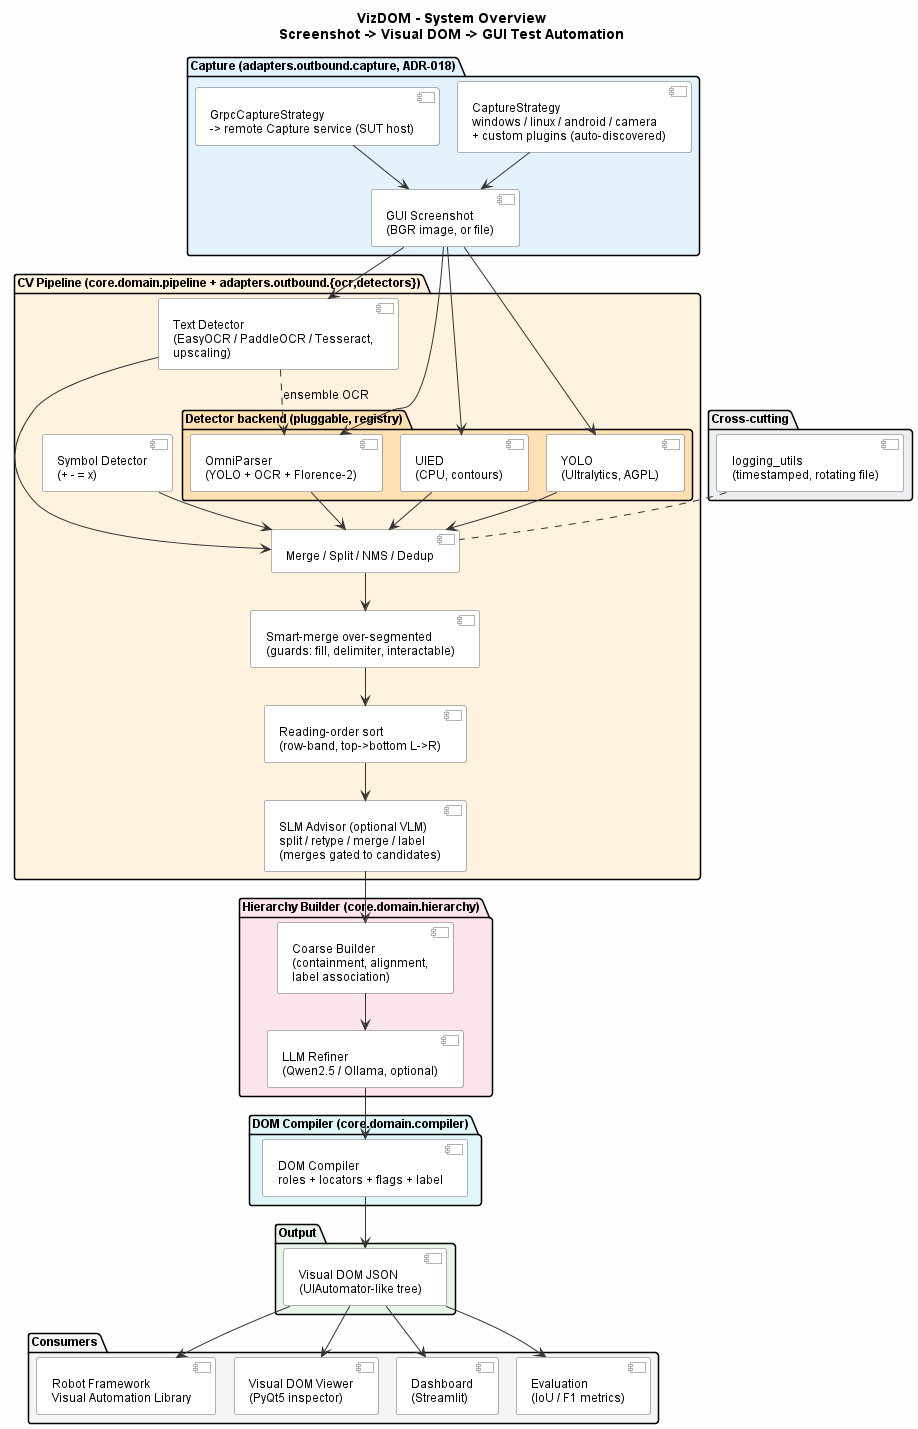
\includegraphics[width=\linewidth]{System_Overview.png}
  \caption{Screenshot $\rightarrow$ Visual DOM $\rightarrow$ test automation. One parse per screen state; every locate, act and verify step is then a query over the cached tree.}
  \label{fig:overview}
\end{figure}

\subsection{Detectors}
Three backends are compared. \emph{UIED} \cite{xie2020uied} is the classical baseline and runs on a CPU. \emph{OmniParser} \cite{omniparser2024} is the monolith: its YOLO detector, OCR and Florence-2 captioner, with VizDOM inferring button, input field, checkbox and icon roles from interactivity, geometry and caption. The \emph{modular} backend takes OmniParser's YOLO as stage one, VizDOM's own OCR as stage two and a port of OmniParser's fusion, with the captioner off; it was built to reproduce the monolith's outcome at a fraction of its parse time, and the benchmark tests that claim.

\subsection{The locator contract}
A locator (\code{text=}, \code{role=}, spatial relations, or combinations) is resolved against the DOM to a set of elements. The contract is \emph{exactly one}: an action with zero or several matches fails with the candidate list, a verification with zero matches fails. This is what makes an absent target fail by construction and what makes a wrong parse visible, since a fragmented or duplicated element produces several matches and stops the step. The price is paid on the clicking side: a caption the OCR cannot read, or a table digit that occurs in a dozen cells, is a miss.

\subsection{The description locator}
\label{sec:desc}
Property locators are deterministic but brittle exactly where perception is weakest. A \code{desc=} locator therefore lets the tester state intent, \code{desc="settings button"}, and imports the grounder paradigm into the parser system with the DOM kept as the source of truth. Resolution escalates through a configurable chain, each tier cheaper and more deterministic than the next, stopping at the first confident hit:
\begin{itemize}
  \item \emph{Lexical over DOM} (no model). Tokens of the description are scored against each element's label, text and hint (weight 2), role words such as ``button'' or ``field'' against its role (weight 1), and positional words against its normalised centre (weight 0.5). The top element is accepted only if its score clears a floor \emph{and} a margin over the runner-up; a tie escalates rather than guesses.
  \item \emph{SLM over DOM}. A small text model (\code{qwen2.5:3b} \cite{qwen25} through Ollama \cite{ollama}, temperature 0) is given a compact table of the candidates and the description and returns an element id with a confidence; the id is validated against the DOM, so a hallucinated id is rejected, and a confidence below 0.5 or a null id declines.
  \item \emph{VLM over image}. The candidates are drawn as numbered boxes on the screenshot (Set-of-Mark \cite{som2023}) and a vision model (\code{qwen2.5vl:3b} \cite{qwen25vl}) is asked which number matches, with null allowed; the answer is a DOM element by construction.
\end{itemize}
Candidates for the model tiers are the top eight of the lexical ranking, or the whole pool when nothing scored. Positional words are enforced geometrically before any model is consulted, because a 3B model confidently called a top-left element ``top right'' in development. The chain is set in configuration (the default is lexical then SLM; CI can pin lexical alone; the vision tier is opt-in), every resolution records which tier answered, and when no tier answers the result lists every tier's own verdict. The design intent is economic: parse once, resolve the easy majority without a model, and ground only the long tail.

% The tier-chain flow chart (report/figures/Desc_Grounding.png) is too dense for a
% column; redraw as a three-box figure if a figure is wanted here.

% =====================================================================
\section{Experimental Setup}
\label{sec:setup}
% =====================================================================
We ask four questions. \textbf{RQ1} How accurately do the systems click? \textbf{RQ2} How well do they judge, and in particular how often do they pass an absent target? \textbf{RQ3} What does each cost per step? \textbf{RQ4} What does VizDOM's own language tier add, and does the oracle property survive putting a model in the loop?

\subsection{Columns}
Seven primary columns, all on the same 514 steps: VizDOM with UIED, OmniParser and the modular backend, resolving the \code{text=} locator; ELAM-7B, UI-TARS-1.5-7B and Aria-UI in bf16 with greedy decoding; and VizDOM-modular resolving the description through the production chain (lexical then SLM). Three further columns pin the chain for RQ4: the SLM alone over the full DOM table, the VLM alone over a Set-of-Mark overlay of the DOM (capped at 20 marks in DOM order), and the VLM behind the lexical shortlist, as production would run it.

\subsection{Hosts and repeatability}
All model columns ran on rented single-GPU hosts with a scripted kit (setup, prefetch, preflight, sweep) and no manual intervention; Table~\ref{tab:runs} lists the runs. Aria-UI's weights (about 50~GB in bf16; its mixture-of-experts layers are not quantised by the 4-bit path, which runs out of memory on a 24~GB card) did not fit the 48~GB card of the main run and were measured on a 96~GB card two hours later with the same manifest and adapter. The language-tier columns ran on a third host, with the plain modular column repeated as a control. Every result file records the dataset id, the commit and the per-step outcome. The VizDOM columns are bit-identical across all hosts and runs; the grounders moved by 3 (ELAM) and 6 (UI-TARS) steps between GPU generations with greedy decoding, about one point of noise on their figures.

\begin{table}[t]
  \centering\scriptsize\setlength{\tabcolsep}{3pt}
  \caption{Runs. All on Vast.ai single-GPU rentals; commits are of the public repository. $^\ast$Columns of these runs are compared across hosts on accuracy only; their latencies are quoted per host.}
  \label{tab:runs}
  \resizebox{\linewidth}{!}{%
  \begin{tabular}{@{}llll@{}}
    \toprule
    Run & GPU & Commit & Columns \\
    \midrule
    3 & RTX 6000 Ada, 48\,GB & \code{82f0b45} & VizDOM $\times$3, ELAM, UI-TARS \\
    3a$^\ast$ & RTX PRO 6000 Blackwell, 96\,GB & \code{411873c} & Aria-UI \\
    4$^\ast$ & RTX PRO 5000 Blackwell, 48\,GB & \code{3fb0924} & control, \code{desc=} $\times$3 \\
    5$^\ast$ & RTX PRO 5000 Blackwell, 48\,GB & \code{c03c438} & control, \code{desc=} $\times$2 \\
    \bottomrule
  \end{tabular}}
\end{table}

\subsection{Software}
Python 3.12; transformers 4.49.0 for VizDOM, OmniParser and UI-TARS, 4.47.1 in a second environment for ELAM's Molmo code and Aria-UI; the 3B models of the language tier served by Ollama on the same host. ELAM uses its model-card grounding and verdict prompts; UI-TARS and Aria-UI use their model-card grounding prompts and the existence proxy for verdicts. No sampling seeds are involved, since all decoding is greedy.

% =====================================================================
\section{Results}
\label{sec:results}
% =====================================================================
Table~\ref{tab:main} is the headline table.

\begin{table*}[t]
  \centering\footnotesize\setlength{\tabcolsep}{4pt}
  \caption{Lifecycle benchmark, 514 steps over 44 states (213 actions, 213 positive and 88 negative verifications). Shaded rows are VizDOM. Cost: for VizDOM, one-off load and per-state parse, amortised per step over the suite; for the grounders, median inference per step. $^\dagger$Measured on the 96\,GB host (run 3a): accuracy comparable, latency from another host. $^\ddagger$Language-tier rows (runs 4--6): the modular control reproduced run 3 on 514 of 514 steps in every run; cost is the resolver time on top of the parse. The default chain is quoted from run 6 (after the shortlist fix of Section~\ref{sec:rq4}; run 4: 0.930 / 0.954 / 0.003), the two single-tier rows from run 4 (run 6 repeated them with a prompt change that is discussed in the text). $^\S$Run 6; 80 of the 116 vision calls of this row were refused by the model server and are scored as misses; the verify-side figures rest on the 30 negatives that were answered (run 5: 0.930 / 0.691 / 0.113 with 68 refused and 34 of 40 passed).}
  \label{tab:main}
  \resizebox{\textwidth}{!}{%
  \begin{tabular}{@{}llcccc l@{}}
    \toprule
    Executor & Weights & Action-hit & Verify acc. & False-pass (of 88) & All correct & Cost \\
    \midrule
    \rowcolor{gray!12} VizDOM + UIED, \code{text=} & CV, no model & 0.822 & 0.934 & \textbf{0.000} (0) & 0.887 & 2.6\,s + 0.39\,s/state = 0.04\,s/step \\
    \rowcolor{gray!12} VizDOM + OmniParser, \code{text=} & CV + Florence-2 & 0.883 & 0.934 & \textbf{0.000} (0) & 0.912 & 8.1\,s + 1.02\,s/state = 0.10\,s/step \\
    \rowcolor{gray!12} VizDOM modular, \code{text=} & CV, captioner off & 0.883 & 0.934 & \textbf{0.000} (0) & 0.912 & 4.2\,s + 0.62\,s/state = 0.06\,s/step \\
    \rowcolor{gray!12} VizDOM modular, \code{desc=} lexical$\rightarrow$SLM$^\ddagger$ & + qwen2.5:3b & 0.934 & \textbf{0.964} & \textbf{0.000} (0) & \textbf{0.951} & parse + 0.03\,s/step (116 model calls) = 0.10\,s/step \\
    \rowcolor{gray!12} \quad \code{desc=} SLM only$^\ddagger$ & qwen2.5:3b & 0.634 & 0.877 & 0.020 (6) & 0.776 & parse + 0.21\,s/step (514 calls) \\
    \rowcolor{gray!12} \quad \code{desc=} VLM only$^\ddagger$ & qwen2.5vl:3b & 0.117 & 0.365 & 0.076 (23) & 0.263 & parse + 0.49\,s/step (514 calls) \\
    \rowcolor{gray!12} \quad \code{desc=} lexical$\rightarrow$VLM$^{\ddagger\S}$ & qwen2.5vl:3b & 0.925 & 0.714 & 0.057 (17) & 0.809 & parse + 0.6\,s per call (116 calls) \\
    ELAM-7B & bf16, 7B & 0.930 & 0.704 & 0.286 (86) & 0.798 & 4.00\,s/step (514 inferences) \\
    UI-TARS-1.5-7B & bf16, 7B & 0.944 & 0.801 & 0.199 (60) & 0.860 & 2.72\,s/step (514 inferences) \\
    Aria-UI$^\dagger$ & bf16, 25B MoE & \textbf{0.962} & 0.708 & 0.292 (88) & 0.813 & 1.57\,s/step (514 inferences) \\
    \bottomrule
  \end{tabular}}
\end{table*}

\subsection{RQ1: clicking}
The three grounders click better than VizDOM resolving exact text: Aria-UI by 8 points over the OmniParser and modular backends, UI-TARS and ELAM by 5 to 6, all of them by 11 to 14 over UIED. The two kinds of miss differ. Every VizDOM miss is a \emph{resolution} miss under the exactly-one contract: 20 steps are captions the OCR cannot read (the placeholder ``Search\ldots'' read without its dots, a path-like value, a few small buttons) and are the same 20 steps in all three detector columns; four are data-table digits that match 12 to 18 cells; UIED adds 12 fragmentation duplicates of its own. The grounders' misses are mislocated points: data-table pagination for ELAM (8 of its 15), login checkboxes and icon buttons for UI-TARS, input fields for Aria-UI. The modular backend reproduces the OmniParser monolith on all 514 steps at 61\,\% of its parse time, which is the parity it was designed for.

\subsection{RQ2: the oracle}
The picture inverts on the oracle question. Asked whether a control that is not on the screen is visible, Aria-UI says PASSED in 88 of 88 cases, ELAM in 86 of 88, UI-TARS in 60 of 88. ELAM's native verdict mode rationalises the unknown label onto a nearby element and then confirms it; the two proxied grounders ground a point for a label that does not exist. VizDOM never does, because the exactly-one contract requires a match before anything is reported present. Its 20 verification errors are all in the conservative direction, a present caption reported FAILED because OCR misread it, which stops the test and summons a person. Table~\ref{tab:verify} shows the three outcomes side by side. The best clicker is the worst oracle, and the difference is structural: a per-step grounder is trained to always produce an answer, whereas a resolved DOM can say no.

\begin{table}[t]
  \centering\scriptsize\setlength{\tabcolsep}{4pt}
  \caption{Outcome of the 301 verification steps. False fail: a true statement rejected (cheap, the test stops). False pass: an absent target accepted (the failure a suite cannot see).}
  \label{tab:verify}
  \resizebox{\linewidth}{!}{%
  \begin{tabular}{@{}lccc@{}}
    \toprule
    Executor & Correct & False fail & False pass \\
    \midrule
    VizDOM, \code{text=} (any of the three detectors) & 281 & 20 & \textbf{0} \\
    VizDOM, \code{desc=} lexical$\rightarrow$SLM (run 6) & \textbf{290} & 11 & \textbf{0} \\
    UI-TARS-1.5-7B & 241 & 0 & 60 \\
    ELAM-7B (native verdict) & 212 & 3 & 86 \\
    Aria-UI & 213 & 0 & 88 \\
    \bottomrule
  \end{tabular}}
\end{table}

\subsection{RQ3: cost}
Amortised over this suite, VizDOM with OmniParser spends 53\,s in total (8.1\,s load plus 44 parses) for 514 steps, about 0.10\,s per step, and the modular backend 0.06\,s; the grounders spend 1.57 to 4.00\,s on every step, 15 to 39 times more for OmniParser and 26 to 65 times more for the modular backend. The ratio depends on how many steps a suite runs against each screen, here about twelve; a suite that visited each screen once would narrow the gap to parse time against inference time. Regression suites revisit the same screens constantly. Aria-UI is the cheapest grounder per step despite being the largest model, because only 3.9B of its parameters are active per token and it ran on a faster card; grounder latency is host-dependent (UI-TARS 1.68\,s per step on an RTX 4090 host against 2.72\,s on the RTX 6000 Ada) and should be quoted as a range.

\subsection{RQ4: the language tier}
\label{sec:rq4}
The \code{text=} rows compare VizDOM \emph{without} its language tier against grounders that are all language tier, and make its zero false-pass partly structural, since a nonsense caption can never match OCR output. Runs 4 to 6 resolve every step a third way, as a description through the \code{desc=} chain over the same modular DOM, with the chain pinned per row; the plain modular column was repeated as a control in each run and reproduced run 3 on all 514 steps. Table~\ref{tab:tiers} shows which tier answered.

\begin{table}[t]
  \centering\scriptsize\setlength{\tabcolsep}{4pt}
  \caption{Which tier answered each of the 514 steps, per pinned chain and run. ``none'' is the correct answer for the 88 negatives and a miss otherwise. ``error'': the model server refused the call; run 4's harness recorded the same refusals as ``none''.}
  \label{tab:tiers}
  \begin{tabular}{@{}lrrrrr@{}}
    \toprule
    Chain & lexical & SLM & VLM & none & error \\
    \midrule
    lexical$\rightarrow$SLM (default), run 6 & 398 & 6 & -- & 110 & 0 \\
    \quad run 4 & 398 & 3 & -- & 113 & 0 \\
    SLM only, run 4 & -- & 372 & -- & 142 & 0 \\
    \quad run 6, explanatory prompt & -- & 459 & -- & 55 & 0 \\
    VLM only, 20-mark overlay, run 4 & -- & -- & 113 & 401 & 0 \\
    \quad run 6 & -- & -- & 101 & 19 & 394 \\
    lexical$\rightarrow$VLM, run 5 & 398 & -- & 40 & 8 & 68 \\
    \quad run 6 & 398 & -- & 23 & 13 & 80 \\
    \bottomrule
  \end{tabular}
\end{table}

\paragraph{The production chain} reaches action-hit 0.934, one step above ELAM, the best verification accuracy of the table (0.964) and no false pass in 88 (run 6; the run-4 measurement it was fixed from is described next). The lexical tier answers 398 of the 514 steps without a model, in 0.2\,ms each. The eleven steps gained over \code{text=} are exactly the OCR-noisy captions that exact text cannot match but token overlap plus the role word can: the placeholder ``Search\ldots'' (seven steps) and path-like values such as \code{APAC\textbackslash USER01}. The one loss is a table digit where the margin between repeated digits is zero. The 13 remaining action misses are the OCR floor, nine captions never read at all and four repeated digits. The text model is consulted on the 116 steps the scoring cannot settle (the 88 negatives and 28 positives). In run 4 it answered three, and its one error was the grounders' failure in miniature, ``Purple Elephant button'' rationalised onto a \emph{Retry} button at confidence 0.85, while it declined the other 87 negatives. The error has a mechanical cause: the dialog's other button is a caption OCR never read, so the lexical ranking scored exactly one element and the model was handed a one-row table, which turns ``which of these matches?'' into ``is this it?''; with two rows the same model declines on the same phrase. The resolver now pads the shortlist to at least three candidates, and run 6 confirms it: the same step declines at confidence 0.00, all 88 negatives are declined, and the padded list lets the model answer six calls instead of three, one of them a new hit (a \emph{Save} button whose caption OCR read as a single letter). Of the 514 outcomes, 509 are identical to run 4 and the other five are gains. One of those gains is instructive: ``Cancel button'' on the same dialog, the unread caption itself, which the model resolved to the dialog's close icon. The action step stays a miss, but the verify step counts as correct, because a positive verification asks only whether some element was confidently resolved. A wrong-element pass on a true statement is invisible to verification accuracy and is caught by action-hit; the two metrics are complementary for that reason.

\paragraph{The text model alone} over the full DOM table (30 to 110 rows) is a poor grounder: 0.634, picking a confidently wrong and semantically unrelated element on 49 of its 78 action misses (``Prev button'' $\rightarrow$ a static text \emph{John Doe}) and passing six absent targets. The lexical tier in front of it is what turns it into a 0.934 column: it answers the easy 77\,\% itself and hands the model a shortlist of eight. Run 6 repeated this row with a prompt that spelled out the null rule (``answer null unless an element's text or role clearly corresponds; a matching role alone is not a match'') and the column got \emph{worse}: 38 false passes instead of six, at confidence 1.00, with the rule quoted back as the justification (``role=button text='Files''' for ``Frobnicate button''). Reproduced offline against the same model with the DOMs the run had parsed: over the whole table the explanatory wording answers six of six nonsense captions and the plain wording one, and over a padded shortlist of three to five rows both decline all six. A 3B model given a long list and a rule copies the rule; given a short list it applies it. The wording was reverted; what carries the oracle is the length of the list, not the prompt.

\paragraph{The vision model alone} measures the harness more than the model. The overlay draws at most 20 marks in DOM order and, with no shortlist, fewer than half of the targets are among them on a DOM with a median of 33 elements per state. On 30 of 44 states the model gave no usable answer in run 4; run 6, whose harness records a refused call as an error, shows that those 30 states were the model-server failure described below, which run 4 had recorded as ``none''. On the 14 states where it did answer it hit 25 of 45 actions (24 of 44 in run 6) and passed all 23 negatives it was asked in run 4, at confidence 0.95 to 1.00; in run 6, with null offered explicitly in the prompt, it passed 13 of 30.

\paragraph{The vision model behind the shortlist} is the experiment that matters, because it is how production would use the tier. It hands the model the 116 steps the lexical tier cannot settle, each with at most eight marks. The row is partial on the action side: for two minutes in the middle of the column the model server answered HTTP 500 to every call, 68 of the 116 (10 actions, 10 positive and 48 negative verifications), and the runner records them as errors, scored as misses and wrong verdicts, rather than as quiet ``no match'' results that would have flattered the column. On the 48 calls that went through, the model behaved like the grounders. Asked about a nonsense caption with a numbered overlay in front of it, it answered a mark on 34 of 40 negatives at confidence 0.90 to 0.99, 22 of them ``mark 1'', and declined six. Of its four action answers one hit. The chain therefore keeps the lexical tier's hits (0.930) and loses the oracle: false-pass 0.113 as measured, which is also the floor had every errored negative been declined, and about 0.25 had they followed the answered rate. Run 6 repeated the column with null offered explicitly in the prompt: 80 of 116 calls refused, and on the 30 negatives answered the model passed 17 and declined 13 (0.925 / 0.714 / 0.057), 57\,\% against 85\,\%, so the wording helps a vision model where it hurts the text model, and the tier is still far from an oracle. The text model, asked the same kind of question over the same shortlist, declines 88 of 88. The refusals are not a server outage: in run 4 (hidden as ``none''), run 5 and both run-6 vision columns the first refused call is the eleventh of the column, the same step, and the refusals cover the same block of states on a given card regardless of whether the column makes 116 or 514 calls. Replaying the calls offline against the same model, with the server's reply kept, names them: \emph{prediction aborted, token repeat limit reached}, the serving layer's guard against a model that loops. On these Set-of-Mark prompts the 3B vision model at temperature~0 either answers the JSON or emits one digit until it is cut off, and which prompts collapse depends on the image and the card's numerics, not on context length (2\,785 prompt tokens, no truncation at any window) or on the request path. The errored steps are therefore the steps on which the vision model produced no answer at all, and the answered subset is the subset it did not loop on. \todo{Re-measure both vision rows with the server log kept and a looping guard in the client; try a 7B vision model.}

This is the second half of the argument. The oracle property of Table~\ref{tab:main} is not a property of having no model in the loop, since the production chain has one and keeps it; nor of model size, since the two models that behave oppositely are both 3B. It is a property of \emph{what the model is asked to do and what it can answer}. A text model asked to pick from a \emph{short} table with an explicit null option, with its answer validated against the DOM and gated by a confidence floor, declines; the same text model over the whole DOM, or a vision model over an image with numbered boxes, does not, and no amount of shortlist in front of the vision model changes that. The tier order in the chain is therefore load-bearing, and so is the length of the list: the deterministic tier answers the majority and shortens the list, the model that can say no handles the tail, and the model that cannot stays out of any chain used for verification.

\subsection{Stability}
Between two runs on different cards (RTX 4090 and RTX 6000 Ada) the OmniParser column reproduced on 514 of 514 steps, and the modular control reproduced on all 514 across four further rentals and commits; every change in a VizDOM figure between runs is accounted for by a code change. ELAM and UI-TARS moved on 3 and 6 steps between GPU generations with greedy decoding, bf16 kernels differing across cards; repeated on the same card model (run 6 against run 3) both reproduced on 514 of 514 steps. Grounder figures therefore carry about one point of noise across hardware and none on a given card; VizDOM's carry none.

% =====================================================================
\section{Threats to Validity}
\label{sec:threats}
% =====================================================================
\paragraph{Synthetic screens} All 44 states come from the project's generator. Real applications have denser, noisier layouts and themed widgets; absolute scores will differ, and the detector columns in particular would lose on OCR. The direction of the oracle finding does not depend on the screens: a grounder passes an absent target because it produces a point for any instruction, which is a property of the model, not of the screen. \todo{Real-application states in the same schema are the planned extension; add their rows here before submission.}

\paragraph{Nonsense negatives} The absent captions are nonsense words, which an exact-text DOM can never partially match, favouring VizDOM, and which a model that reads the screen might reasonably be expected to reject, yet mostly did not. Plausible-but-absent labels (``Export'' on a screen with ``Import'') would test VizDOM's OCR and lexical tier as well; this is planned as defect injection. \todo{Add the harder negative set.}

\paragraph{Generated descriptions} The \code{desc=} descriptions are caption plus role word, the lexical tier's ideal input; a tester's own wording would exercise the model tiers more. The production chain's 0.934 is an upper bound for this phrasing. \todo{Human-written or paraphrased descriptions.}

\paragraph{Proxied verdicts} UI-TARS and Aria-UI have no verdict mode, so ``grounded a point'' counts as PASSED. ELAM's native verdict is the fairer comparison and still passes 86 of 88 absent targets, so the proxy is not what drives the finding.

\paragraph{Two cards, no seeds} There are no estimates across sampling seeds since decoding is greedy; the cross-card difference gives about one point of uncertainty for the grounders, and a repeat on the same card model reproduced them exactly. \todo{Repeat the grounder columns on a third card.}

\paragraph{Small models in the language tier} The 3B models are what fits beside the pipeline on one card; a 7B text or vision model may behave differently, in either direction. Both vision-chain columns (runs 5 and 6) are partial on the action side because of the model-server failure, and their action-side question, whether a vision model recovers the OCR floor, is open. The single-tier text row is quoted from run 4 because run 6 repeated it with a prompt that regressed it. \todo{Rerun the vision-chain and SLM-only columns with the server log kept; try 7B tiers.}

\paragraph{OCR, not the DOM logic, caps VizDOM's verification accuracy} The 20 false fails are the same 20 captions in all three detector columns and in every run; a better OCR would move that figure without touching the oracle result.

% =====================================================================
\section{Conclusion}
% =====================================================================
We asked whether a vision--language grounder can serve as a GUI test oracle, and built a benchmark that can tell. On 514 locate--act--verify steps, three state-of-the-art grounders click more accurately than a system that parses the screenshot into a DOM and resolves exact text (0.93--0.96 against 0.88), but pass 60 to 88 of 88 absent targets, where the DOM passes none by construction and costs 15 to 39 times less per step. With a description locator resolved by deterministic scoring first and a small text model only where the scoring is not confident, the DOM system matches the grounders' clicking (0.934), verifies best (0.964) and passes none of the 88 absent targets. Placing a 3B vision model in the same chain keeps the clicking and destroys the oracle (34 false passes in 40 answered negatives, then 17 in 30 with null offered explicitly), and handing the text model the whole DOM instead of a short list does the same (38 in 88), which locates the failure in per-step grounding over an unstructured input rather than in model size or in the absence of a model.

For practitioners the result is a design rule: use perception once per screen to build a structure that can return zero matches, resolve the easy majority of steps deterministically against it, and consult a model only on the tail and only in a form whose answer can be validated against the structure and can be ``none''. For benchmark designers it is a missing column: an agent benchmark that does not contain a step whose correct answer is ``not here'' cannot tell an oracle from an agent.

Future work is the real-world dataset in the same schema, plausible-but-absent negatives, human-written descriptions, repeated runs for error bars, a vision tier that can decline, and a complete measurement of the vision rows once the model-server failure is understood.

\section*{Artifact}
The benchmark generator, the step manifest, the run kit and the result files are in the project repository. \todo{Zenodo DOI for the result tarballs and the manifest; repository URL.}

\bibliographystyle{IEEEtran}
\bibliography{references}

\end{document}
